\documentclass[12pt,aspectratio=169]{beamer}
% Tema y configuración
\usefonttheme{professionalfonts}
\usepackage[utf8]{inputenc}
\usepackage[spanish]{babel}

% Paquetes necesarios
\usepackage{tikz}
\usepackage{pgfplots}
\usepackage{xcolor}
\usepackage{multicol}
\usepackage{textcomp}
\usepackage{siunitx}

\usepackage{amsmath}
\usepackage{amssymb}
\usepackage{graphicx}
\usepackage{fontawesome5} % Para iconos
\usepackage{hyperref}

\usetheme{Madrid}
\usecolortheme{spruce}

\setbeamertemplate{itemize items}[default]
\setbeamertemplate{enumerate items}[default]

% define a darker brown
\definecolor{uwbrown}{HTML}{662200}
% apply dark brown to the item bullet points
\setbeamercolor{item}{fg=uwbrown}
%\usecolortheme[named=uwbrown]{structure}
\usetikzlibrary{shapes,arrows,positioning,decorations.pathmorphing}
\pgfplotsset{compat=1.17}

% Colores personalizados
\definecolor{azuloscuro}{RGB}{25,25,112}
\definecolor{rojoclaro}{RGB}{220,20,60}
\definecolor{verdeclaro}{RGB}{50,205,50}
\definecolor{naranjaclaro}{RGB}{255,140,0}

% Configuración de fuentes más grandes
\setbeamerfont{title}{size=\huge,series=\bfseries}
\setbeamerfont{subtitle}{size=\Large}
\setbeamerfont{frametitle}{size=\Large,series=\bfseries}
\setbeamerfont{framesubtitle}{size=\large}
\setbeamerfont{normal text}{size=\large}
\setbeamerfont{caption}{size=\large}

% Configuración de ecuaciones grandes
\everymath{\displaystyle}

% --- Configuración de Hipervínculos ---
\hypersetup{
	colorlinks=true,
	linkcolor=blue,
	filecolor=magenta,
	urlcolor=teal, % Un color agradable para URLs
	pdftitle={El Efecto Fotoeléctrico},
	pdfpagemode=FullScreen,
}
\newcommand{\KEmax}{KE_{\text{máx}}}
\newcommand{\nuo}{\nu_0}
\newcommand{\lambdao}{\lambda_0}
\newcommand{\funcphi}{\Phi} % O \phi si prefieres la minúscula

\title[]{El Efecto Fotoeléctrico}
\subtitle{Ingeniería en Nanotecnología}
\author{[ruben.velazquez@uteq.edu.mx]}
\institute[UTEQ]{Universidad Tecnológica de Querétaro}
\date{Mayo - Agosto 2025}
\logo{
\includegraphics[width=2cm]{../Imagenes/Logo_uteq}}
% \logo{\includegraphics[height=1.5cm]{/home/jordan/Pictures/wyo_logo_small.png}}
\begin{document}
	
	% --- Diapositiva 1: Título ---
	\begin{frame}
		\titlepage
	\end{frame}
	
	% --- Diapositiva 2: El Enigma Cuántico ---
	\begin{frame}{El Enigma Cuántico}
		\begin{figure}
			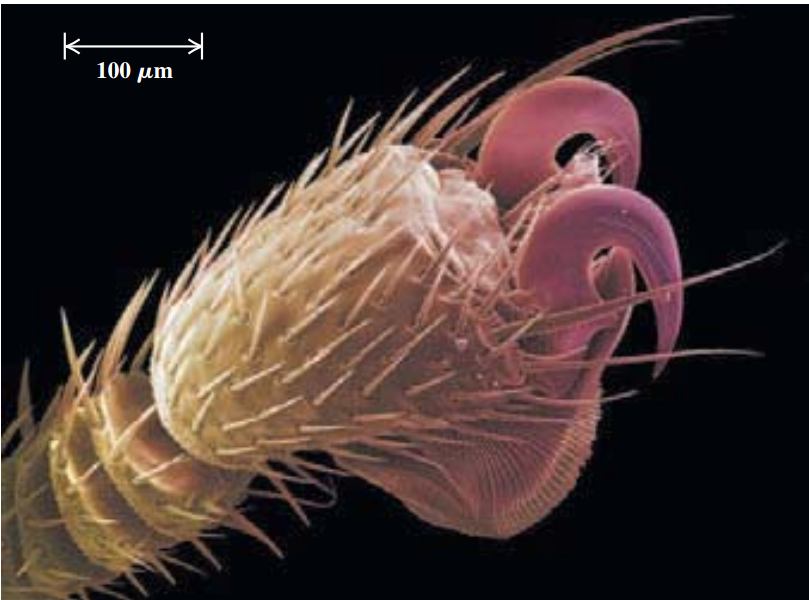
\includegraphics[width=0.6\textwidth]{../Imagenes/mosca} % Reemplaza con tu imagen de la mosca
			\caption{Imagen de una mosca de murciélago obtenida con un haz de electrones (p. 1349).}
		\end{figure}
		
	\end{frame}
	
	\begin{frame}
		\begin{block}{Pregunta Inicial}
			Esta imagen se tomó con un \textbf{haz de electrones}, no de luz.
			\vspace{0.5em}
			¿Qué propiedad de los electrones permite obtener imágenes con un nivel de detalle que la luz visible no puede alcanzar?
		\end{block}
		\begin{flushright}
			\tiny{\textit{Nota para el presentador: Hipótesis de De Broglie (p. 1350) y longitud de onda.}}
		\end{flushright}
	\end{frame}
		% --- Diapositiva 3: La Necesidad de una Nueva Física ---
	\begin{frame}{La Necesidad de una Nueva Física}
		\begin{block}{Más allá del modelo de Bohr}
			\begin{itemize}
				\item El modelo de Bohr fue un gran avance, pero era inconsistente: mezclaba ideas clásicas y cuánticas.
				\item No podía explicar átomos más complejos que el hidrógeno.
				\item Como dice el texto: \textit{"Se necesitaban desviaciones más drásticas respecto de los conceptos clásicos."} (p. 1349)
			\end{itemize}
		\end{block}
		\pause
		La solución es la \textbf{Mecánica Cuántica}, una teoría que describe la materia no como partículas puntuales, sino como \textbf{ondas}.
	\end{frame}

	\begin{frame}{Recordando las Ondas Clásicas (Parte 1)}
		\begin{block}{Antes de lo cuántico, recordemos lo clásico}
			Pensemos en una onda simple que todos conocemos: \textbf{una onda en una cuerda de guitarra.}
		\end{block}
	\begin{figure}
		\centering
		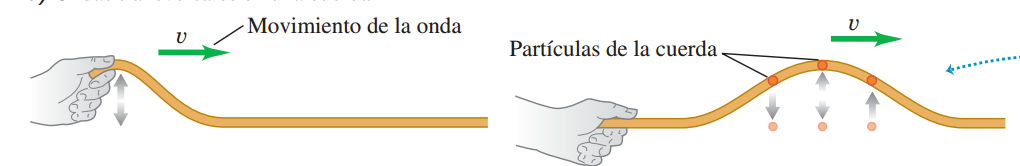
\includegraphics[width=0.7\textwidth]{../Imagenes/cuerda} 
		\caption{Onda en una cuerda}
	\end{figure}
	\textbf{Pregunta:} ¿Cómo describimos matemáticamente esta onda?
\end{frame}

	\begin{frame}{Recordando las Ondas Clásicas (Parte 2)}
		\begin{block}{La Función de Onda Clásica}
			Usamos una \textbf{función de onda clásica} para describir el desplazamiento $y$ de cada punto $x$ de la cuerda en cualquier instante $t$:
			\begin{center}
				\Large $y(x, t)$
			\end{center}
			\vspace{1em}
			\textbf{¿Qué información contiene $y(x, t)$?}
		\begin{itemize}
			\item La \textbf{forma} de la onda en el espacio.
			\item La \textbf{amplitud} (relacionada con la energía de la onda).
			\item La \textbf{velocidad} de cualquier punto de la cuerda.
			\item ¡Contiene \textbf{TODA la información} sobre el estado de la cuerda!
		\end{itemize}
	\end{block}
	Esta idea de una función que describe completamente un sistema es clave.
	\end{frame}
	
	\begin{frame}{Analogía Visual: De lo Clásico a lo Cuántico}
		\begin{block}{Construyendo un Puente Conceptual}
			\begin{tabular}{|m{0.45\textwidth}|m{0.45\textwidth}|}
			
				\centering \textbf{Mundo Clásico (Cuerda)} & \centering \textbf{Mundo Cuántico (Electrón)} \\
			
				\textbf{Objeto:} Cuerda vibrante & \textbf{Objeto:} Partícula (ej. electrón) \\
				\textbf{Descripción:} Desplazamiento $y$ & \textbf{Descripción:} ??? \\
				\textbf{Función:} \large $y(x, t)$ & \textbf{Función:} \large $\Psi(x, y, z, t)$ \\
				\textbf{Propósito:} Describe la forma y movimiento de la cuerda. & \textbf{Propósito:} Describe el \textbf{estado cuántico} de la partícula. 
			\end{tabular}
		\end{block}
		\vspace{1em}
		Vamos a usar la misma idea de una "función de onda" para describir el electrón, pero su significado será diferente y más profundo.
\end{frame}
	
	\begin{frame}{¿Qué es la Función de Onda ($\Psi$)?}
		\begin{block}{El lenguaje de las ondas cuánticas}
			Así como una onda en una cuerda se describe por $y(x, t)$, una partícula en mecánica cuántica se describe por su \textbf{Función de Onda}:
			\begin{center}
				\Huge $\Psi(x, y, z, t)$
			\end{center}
			\begin{itemize}
				\item Es una función matemática que \textbf{contiene toda la información posible} sobre la partícula.
				\item \textbf{¡CUIDADO!} No es una onda física en un medio material. Es una \textbf{onda de probabilidad} (p. 1362).
			\end{itemize}
		\end{block}
	\end{frame}
	
	\begin{frame}{Un Caso Especial: Estados Estacionarios}
		\begin{block}{Simplificando el problema}
			Un \textbf{estado estacionario} es un estado donde la partícula tiene una \textbf{energía definida y constante ($E$)}.
			\vspace{0.5em}
			En este caso, la función de onda se puede separar:
			\begin{equation*}
				\Psi(x, y, z, t) = \psi(x, y, z) \cdot e^{-iEt/\hbar}
			\end{equation*}
			\centering (Ecuación 39.14, p. 1363)
			\vspace{0.5em}
			\begin{itemize}
				\item $\psi(x, y, z)$: Parte espacial (independiente del tiempo).
				\item $e^{-iEt/\hbar}$: Parte temporal (oscilatoria).
			\end{itemize}
		\end{block}
		Nos enfocaremos en la parte espacial, $\psi(x)$, que describe la "forma" de la onda.
	\end{frame}
	
		\begin{frame}{La Gran Pregunta...}
		\begin{alertblock}{Si $\Psi$ es un número complejo, ¿qué significa físicamente?}
			\begin{itemize}
				\item No podemos medir $\Psi$ directamente.
				\item ¿Cómo conectamos esta función matemática abstracta con los experimentos y el mundo real?
			\end{itemize}
		\end{alertblock}
		\begin{figure}
			\centering
			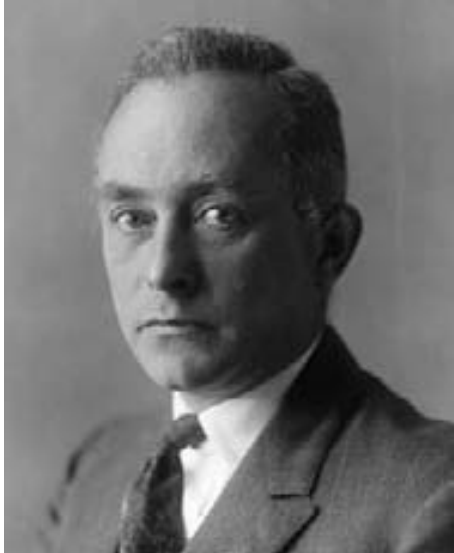
\includegraphics[width=0.3\textwidth]{../Imagenes/MaxBorn} % Reemplaza con imagen de Max Born
			\caption{Max Born (p. 1362).}
		\end{figure}
		\centering La respuesta la dio Max Born en 1926.
	\end{frame}
	\begin{frame}{La Interpretación de Born: Probabilidad}
	El significado físico no está en $\Psi$, sino en el \textbf{cuadrado de su valor absoluto}:
	\begin{center}
		\Huge $|\Psi|^2$
	\end{center}
	\begin{itemize}
		\item $|\Psi|^2$ se conoce como la \textbf{densidad de probabilidad}.
		\item $|\Psi|^2 dV$ es la \textbf{probabilidad} de encontrar la partícula en un pequeño volumen $dV$.
	\end{itemize}
	\vspace{1em}
	\begin{beamercolorbox}[sep=0.3cm,center,wd=\textwidth]{block body alerted}
		\textbf{En resumen: Donde $|\Psi|^2$ es grande, es muy probable encontrar la partícula.}
	\end{beamercolorbox}
	\tiny{\textit{Sugerencia: Dibujar en pizarra $\psi(x)$ vs $|\psi(x)|^2$.}}
\end{frame}	
	
\end{document}